\section{\ttbar~background}
\label{sec:ttbar}

This section describes the estimate
of the contribution of \ttbar~events to the 
background in both the \eejj~and \enujj~channels.
In the \eejj~channel, the \ttbar~contribution
to the total background is estimated from data using 
\emujj~events.  This process is described in Section
\ref{sec:eejjTTbarBkg} 
In the \enujj~channel, the \ttbar~contribution to the total
background is estimated from MC events that have been
rescaled within a control region, as described
in Section \ref{sec:enujjTTbarWJetsBkg}.

\subsection{\ttbar~background in the \eejj~channel} 
\label{sec:eejjTTbarBkg}    


\begin{table}[htb]
  \begin{center}
    \small
    \begin{tabular}{l|c} 
      HLT path & Run number range \\%& \Lint (pb$^{-1}$) \\
      \hline\hline
      \multicolumn{2}{c}{Run2011A} \\
      \hline
      \verb HLT_Mu15_Photon20_CaloIdL_v2  &       160404--161176 \\%& 5.281 \\
      \verb HLT_Mu15_Photon20_CaloIdL_v3  &       161216--163261 \\%& 28.321\\
      \verb HLT_Mu15_Photon20_CaloIdL_v4  &       163269--163869 \\%& 168.613 \\
      \verb HLT_Mu15_Photon20_CaloIdL_v5  &       165088--165633 \\%& 139.026 \\
      \verb HLT_Mu15_Photon20_CaloIdL_v6  &       165970--166967 \\%& 524.904 \\
      \verb HLT_Mu15_Photon20_CaloIdL_v7  &       167039-167913  \\%& 265.663 \\
      \verb HLT_Mu15_Photon20_CaloIdL_v9  &       170249-173198 \\%& 748.931\\  
      \verb HLT_Mu17_Ele8_CaloIdT_CaloIsoVL_v4 &   173236--173692 \\%& 246.527 \\
      \hline
      \multicolumn{2}{c}{Run2011B}  \\
      \hline
      \verb HLT_Mu17_Ele8_CaloIdT_CaloIsoVL_v4 &  175832--178380 \\%& 1698 \\
      \verb HLT_Mu17_Ele8_CaloIdT_CaloIsoVL_v7 &  178420--179889 \\%& 694.789 \\ 
      \verb HLT_Mu17_Ele8_CaloIdT_CaloIsoVL_v8  & 179959--180252 \\%& 117.644 \\

    \end{tabular}
    \caption{HLT paths used to select events in the \emujj~control sample, used for the
      data driven \ttbar~background estimate in the \eejj~channel.}
    \label{tab:emujjHLT}
  \end{center}
\end{table}
 

The contribution of \ttbar~events to the total background in the \eejj~channel 
mainly comes from the process in Equation \ref{eqn:emujj}:
\begin{equation}
  \mbox{\ttbar} \rightarrow \mbox{\PW} \mbox{b} + \mbox{\PW} \mbox{b} \rightarrow \mbox{e} \nu \mbox{b} + \mbox{e} \nu \mbox{b} \rightarrow \mbox{eejj} \quad
  \label{eqn:emujj}
\end{equation} 
This contribution (both in terms of number of events and shape of kinematic distributions) 
is estimated from data using a control sample containing one electron, one muon, and at least two jets.
It should be noted that this \emujj~sample is signal-exclusive: mBRW leptoquark pair production events 
do not produce \emujj~final states, under the assumption of no mixing between 
the generations of leptons and quarks (see assumption {\bf 5} in Section \ref{sec:brw-model}).
The dominant process contributing to this control 
sample is identical to the \ttbar~process described in Equation \ref{eqn:emujj}, except
one of the Ws decays to a muon-neutrino pair instead of an electron-neutrino pair, yielding an \emujj~final state.
In addition to \ttbar~events, 
This \emujj~sample contains
a small (\ContaminationAtTTBARemujj~as derived from MC) contamination of non-\ttbar~events, mainly diboson events.

The events in the \emujj~control region are selected online using unprescaled muon-photon 
or muon-electron triggers.
The exact trigger used depends on the run period, as reported in Table~\ref{tab:emujjHLT}.
The requirements of these triggers may be broken down as follows:
\begin{itemize}
\item Triggers with the word {\tt Mu15} ({\tt Mu17}) in their name require a global muon with $\pt > 15$ (17) GeV in the event.
\item Triggers with the word {\tt Photon20} in their name require an energy cluster in the ECAL with a reconstructed $\et$ greater than 20 GeV.
\item Triggers with the word {\tt Ele8} in their name require an energy cluster in the ECAL with a reconstructed $\et$ greater than 8 GeV.  In addition,
  this energy cluster must be matched to hits in the pixel detector.
\item The word {\tt CaloIdL} in the trigger name implies an identification requirement on the ECAL energy cluster.  
There must not be significant energy deposits in the HCAL cells directly behind the ECAL cluster
(\HoE$ < 0.15$ for electrons in the EB, \HoE$ < 0.10$ for electrons in the EE)
and the shape of the ECAL cluster must be consistent with the shape of clusters typically produced by electrons and photons
(\SigmaiEtaiEta$ < 0.014$ for electrons in the EB, \SigmaiEtaiEta$ < 0.035$ for electrons in the EE).
Similarly, {\tt CaloIdT} implies a 
requirement of \HoE$< 0.10$ (0.075) for electrons in the EB (EE) and a 
requirement of \SigmaiEtaiEta$ < 0.011$ (0.031) for electrons in the EB (EE).
\item The word {\tt CaloIsoVL} implies an energy isolation requirement on the ECAL energy cluster.
Excluding the energy cluster itself, the sum of the energy in the ECAL cells surrounding the energy cluster
must not be greater than 20\% of the electron \et.  The same requirement is placed on the energy
in the HCAL cells.
\end{itemize}

In addition to the trigger requirements described above, the \eejj~preselection and final selection requirements described 
in Section~\ref{sec:eejjSelection} are applied to the \emujj~sample, where the muon is treated as a second electron.  

In MC, before any event reconstruction or selection biases, the \ttbar~process is expected to 
produce twice as many \emujj~events as \eejj~events with the same kinematic properties.
In data, the relation between the number of \eejj~and \emujj~events at any given stage of the selection 
must be corrected for trigger, reconstruction, ID, and isolation efficiencies of leptons.
The number of \eejj~events produced by the \ttbar~process
may be estimated using the number of \emujj~events via Equation \ref{eqn:emujj_vs_eejj_ttbar}:
\begin{equation}
  \mbox{N}_{\mbox{\eejj}}^{\mbox{data}} = \mathcal{C}  \times \mbox{N}_{\mbox{\emujj}}^{\mbox{data}} = \frac{1}{2} \times \frac{\epsilon_{ee}^{trg}}{\epsilon_{e\mu}^{trg}} \times \frac{\epsilon_{e}^{reco/ID/Iso}}{\epsilon_{\mu}^{reco/ID/Iso}} \times \mbox{N}_{\mbox{\emujj}}^{\mbox{data}} 
  \label{eqn:emujj_vs_eejj_ttbar}
\end{equation}
where :
\begin{itemize}
\item$\epsilon_{ee}^{trg}$ is the efficiency
  with which the triggers in Table \ref{tab:eejjDoublePhotEleHLT} 
  select events with two HEEP electrons, as defined in Section \ref{sec:id-electron}.
  This efficiency is taken to be 100\%, as described in Section~\ref{sec:eejjTrigger}.
\item $\epsilon_{e\mu}^{trg}$ is the efficiency with
  which the triggers in Table \ref{tab:emujjHLT} select 
  events with one HEEP electron and one muon passing the tight muon ID, as described
  in Section \ref{sec:id-muon}.  This efficiency is also assumed to be 100\%
\item $\epsilon_{e}^{reco/ID/Iso}$ ($\epsilon_{\mu}^{reco/ID/Iso}$) 
  is the efficiency with which electrons (muons) coming from \emujj events are
  reconstructed and pass the identification and isolation requirements.
  The ratio of these efficiencies is determined from MC by comparing the number of \eejj~events that pass
  the \eejj~preselection with the number of \emujj~events that pass the \eejj~preselection if 
  the muon is treated as a second electron.  The calculation of this ratio is described
  in Equation \ref{eqn:emujj2}:
  \begin{equation}
    \epsilon_{e}^{reco/ID/Iso} / \epsilon_{\mu}^{reco/ID/Iso} = 2 \times \mbox{N}_{\mbox{\eejj}}^{\mbox{MC}} /\mbox{N}_{\mbox{\emujj}}^{\mbox{MC}} = \mbox{\ratioEmuRecoEff} 
    \label{eqn:emujj2}
  \end{equation}
  This assumption is justified in light of the fact that both electron and muon efficiencies are 
  measured to have minimal differences between data and MC~\cite{zprime-2011}.
  The 2\% systematic uncertainty on this ratio 
  comes from the uncertainty on the electron reconstruction efficiency (1.5\%) and
  the uncertainty on the muon reconstruction efficiency (1.0\%).
\end{itemize}
The \ttbar~background prediction is finally obtained by rescaling 
the \emujj~data by the factor \\ $\mathcal{C} = \mbox{\rescaleFactorTTBAReejj}$. 
The \ttbar~contributions in the \eejj~channel shown in the tables and plots 
of this note are obtained using this method.

The number of \ttbar~events passing the \eejj~preselection, estimated using the \emujj~sample, 
is $768 \pm 19$, to be compared with $790 \pm 14$ events obtained directly from MC 
(only statistical uncertainties are shown).
Figure~\ref{fig:st_mej_ttbar_eejj_emuVsMC} shows the comparison 
of \st~and \mej~distributions between the data-driven \ttbar~background 
prediction and the \ttbar~background prediction using MC at \eejj~preselection level.
The agreement is good in both the shape and the normalization. 
    
 \begin{figure}[htbp]
  \begin{center}
    \begin{tabular}{cc}
      \resizebox{7.5cm}{!}{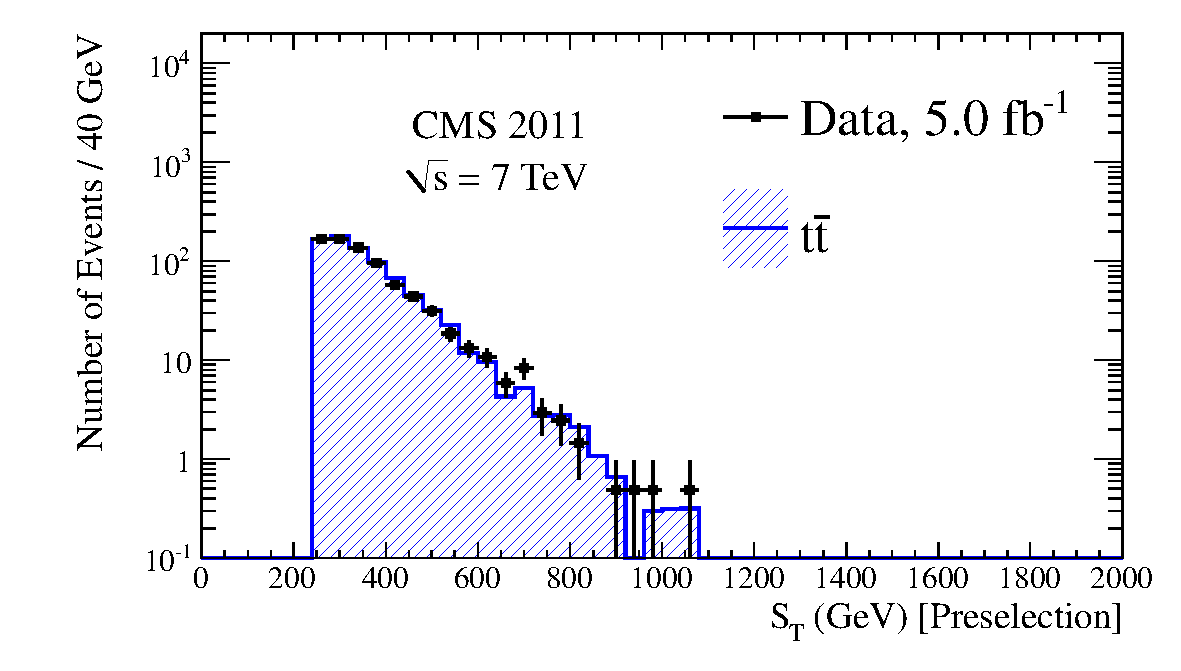
\includegraphics{tex/analysis/backgrounds/fig/sT_PAS_emujj.pdf}} &
      \resizebox{7.5cm}{!}{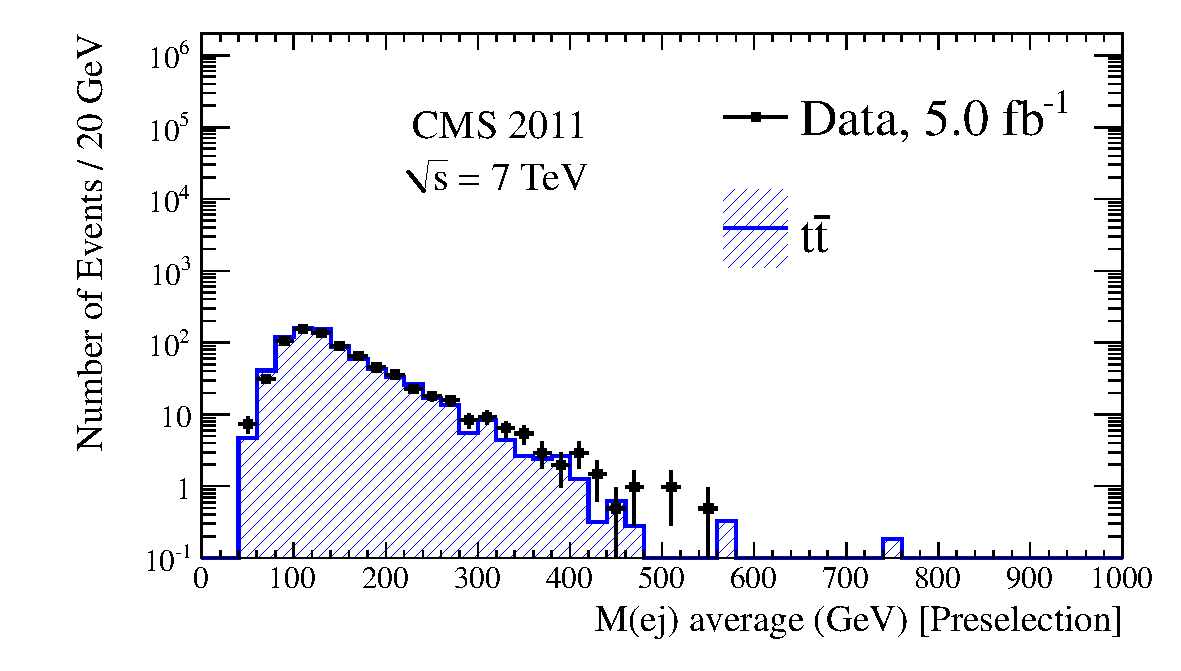
\includegraphics{tex/analysis/backgrounds/fig/Mej_selected_avg_PAS_emujj.pdf}} \\
    \end{tabular}
    \caption{Distributions showing the \st~(left)
             and average \mej~of the two reconstructed leptoquark candidates (right) 
             for \ttbar~background predictions using
             the \emujj~data sample (black) and MC events passing the \eejj~preselection (blue)}
    \label{fig:st_mej_ttbar_eejj_emuVsMC}
  \end{center}
\end{figure}   
   
%        
\subsection{\ttbar~(and \wjets) background in the \enujj~channel} 
\label{sec:enujjTTbarWJetsBkg}

The \ttbar~and \wjets~selection efficiencies in the \enujj~analysis are derived from MC.
The \ttbar~and \wjets~sample normalizations are obtained by comparing data and simulation
after two separate selection criteria: one that enriches the samples with \ttbar~events 
and one that enriches the samples with \wjets~events.

The following selection (selection 1) enriches the samples with \wjets~events, with a contamination of \ContaminationAtWpeak, 
mainly coming from \ttbar~events.  This selection includes events which:
\begin{itemize}
\item Pass \enujj~preselection;
\item Have $50<\mt<110$~GeV;
\item Have less than 5 jets with $\pt>40$~\GeV and $|\eta|<3$.
\end{itemize}

The following selection (selection 2) enriches the samples with \ttbar~events, with a contamination of \ContaminationAtTTBARenujj, mainly coming from \wjets~and QCD multijet events.  This selection includes events which:
\begin{itemize}
\item Pass \enujj~preselection
\item Have $50<\mt<110$~GeV
\item Have at least 5 jets with $\pt>40$~\GeV and $|\eta|<3$
\end{itemize}

The results of these two selections can be used to form a system of equations:

\begin{equation}
\begin{cases}
\mbox{N}_{\mbox{data}}^{\mbox{1}} = \mathcal{R}_{\mbox{\ttbar}} \mbox{N}_{\mbox{\ttbar}}^{\mbox{1}} + \mathcal{R}_{\mbox{\PW}}\mbox{N}_{\mbox{\PW}}^{\mbox{1}} + \mbox{N}_{\mbox{QCD}}^{\mbox{1}}  +  \mbox{N}_{\mbox{Others}}^{\mbox{1}} \\
\mbox{N}_{\mbox{data}}^{\mbox{2}} = \mathcal{R}_{\mbox{\ttbar}} \mbox{N}_{\mbox{\ttbar}}^{\mbox{2}} + \mathcal{R}_{\mbox{\PW}}\mbox{N}_{\mbox{\PW}}^{\mbox{2}} + \mbox{N}_{\mbox{QCD}}^{\mbox{2}}  +  \mbox{N}_{\mbox{Others}}^{\mbox{2}} 
\end{cases}
\end{equation}

where $\mbox{N}_{\mbox{data}}^{\mbox{i}}$, $\mbox{N}_{\mbox{\PW}}^{\mbox{i}}$, $\mbox{N}_{\mbox{Others}}^{\mbox{i}}$, 
$\mbox{N}_{\mbox{\ttbar}}^{\mbox{i}}$, and  $\mbox{N}_{\mbox{QCD}}^{\mbox{i}}$
are, respectively, the number of events in data, the number of events predicted by the \wjets~MC sample before rescaling,
and the number of events predicted by other MC backgrounds (single-top, diboson, etc..),
the number of events predicted by the \ttbar~MC sample before rescaling, 
and the predicted number of QCD multijet events obtained with the method described in Section~\ref{sec:qcd}, passing selection $i$.
Solving the system yields the following rescaling factors for the {\sc MadGraph} \ttbar~and the {\sc Sherpa} \wjets~samples:
\begin{eqnarray}
\mathcal{R}_{\mbox{\ttbar}} = \mbox{\rescaleFactorTTBARenujj}  \\
\mathcal{R}_{\mbox{\PW}} = \mbox{\rescaleFactorWSherpa} .
\end{eqnarray}

For this study all MC samples are normalized using the cross sections listed in Section~\ref{sec:mc-samples}. 
These factors are already included in the \ttbar~and \wjets~MC predictions for the \enujj~channel.
Figure~\ref{fig:manyplots_enujj_ttbarEnriched} shows the distributions of several reconstructed 
quantities for events passing the criteria in selection 2 listed above, after the rescaling factors have been 
applied to the \wjets~and \ttbar~MC. 
A good agreement between data and background prediction is found in the shape of all these distributions.  

\begin{figure}[htbp]
  \begin{center}
    \begin{tabular}{cc}
      \resizebox{7.5cm}{!}{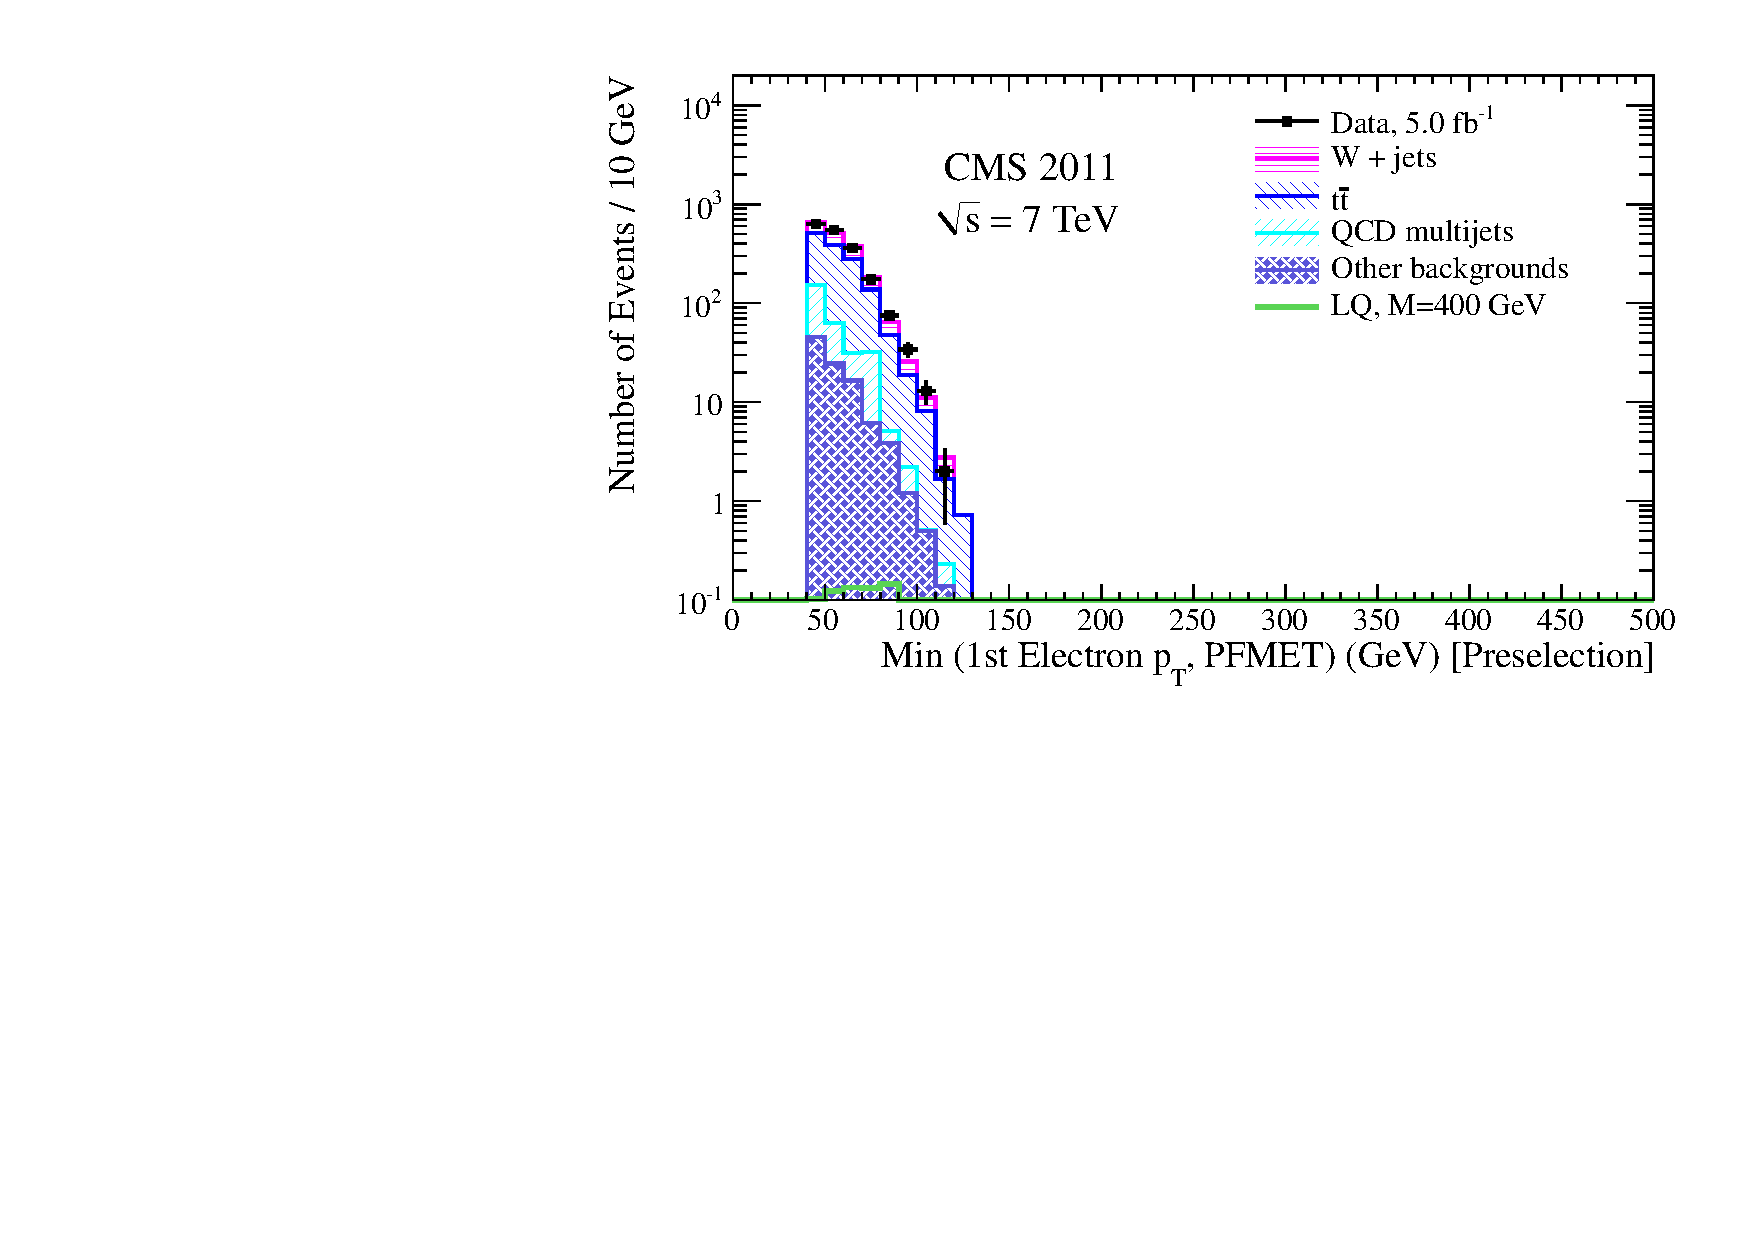
\includegraphics{tex/analysis/backgrounds/fig/minMETPt1stEle_PAS_enujj_TTBarNorm_5Jets_WZSherpaScaled.pdf}} &
      \resizebox{7.5cm}{!}{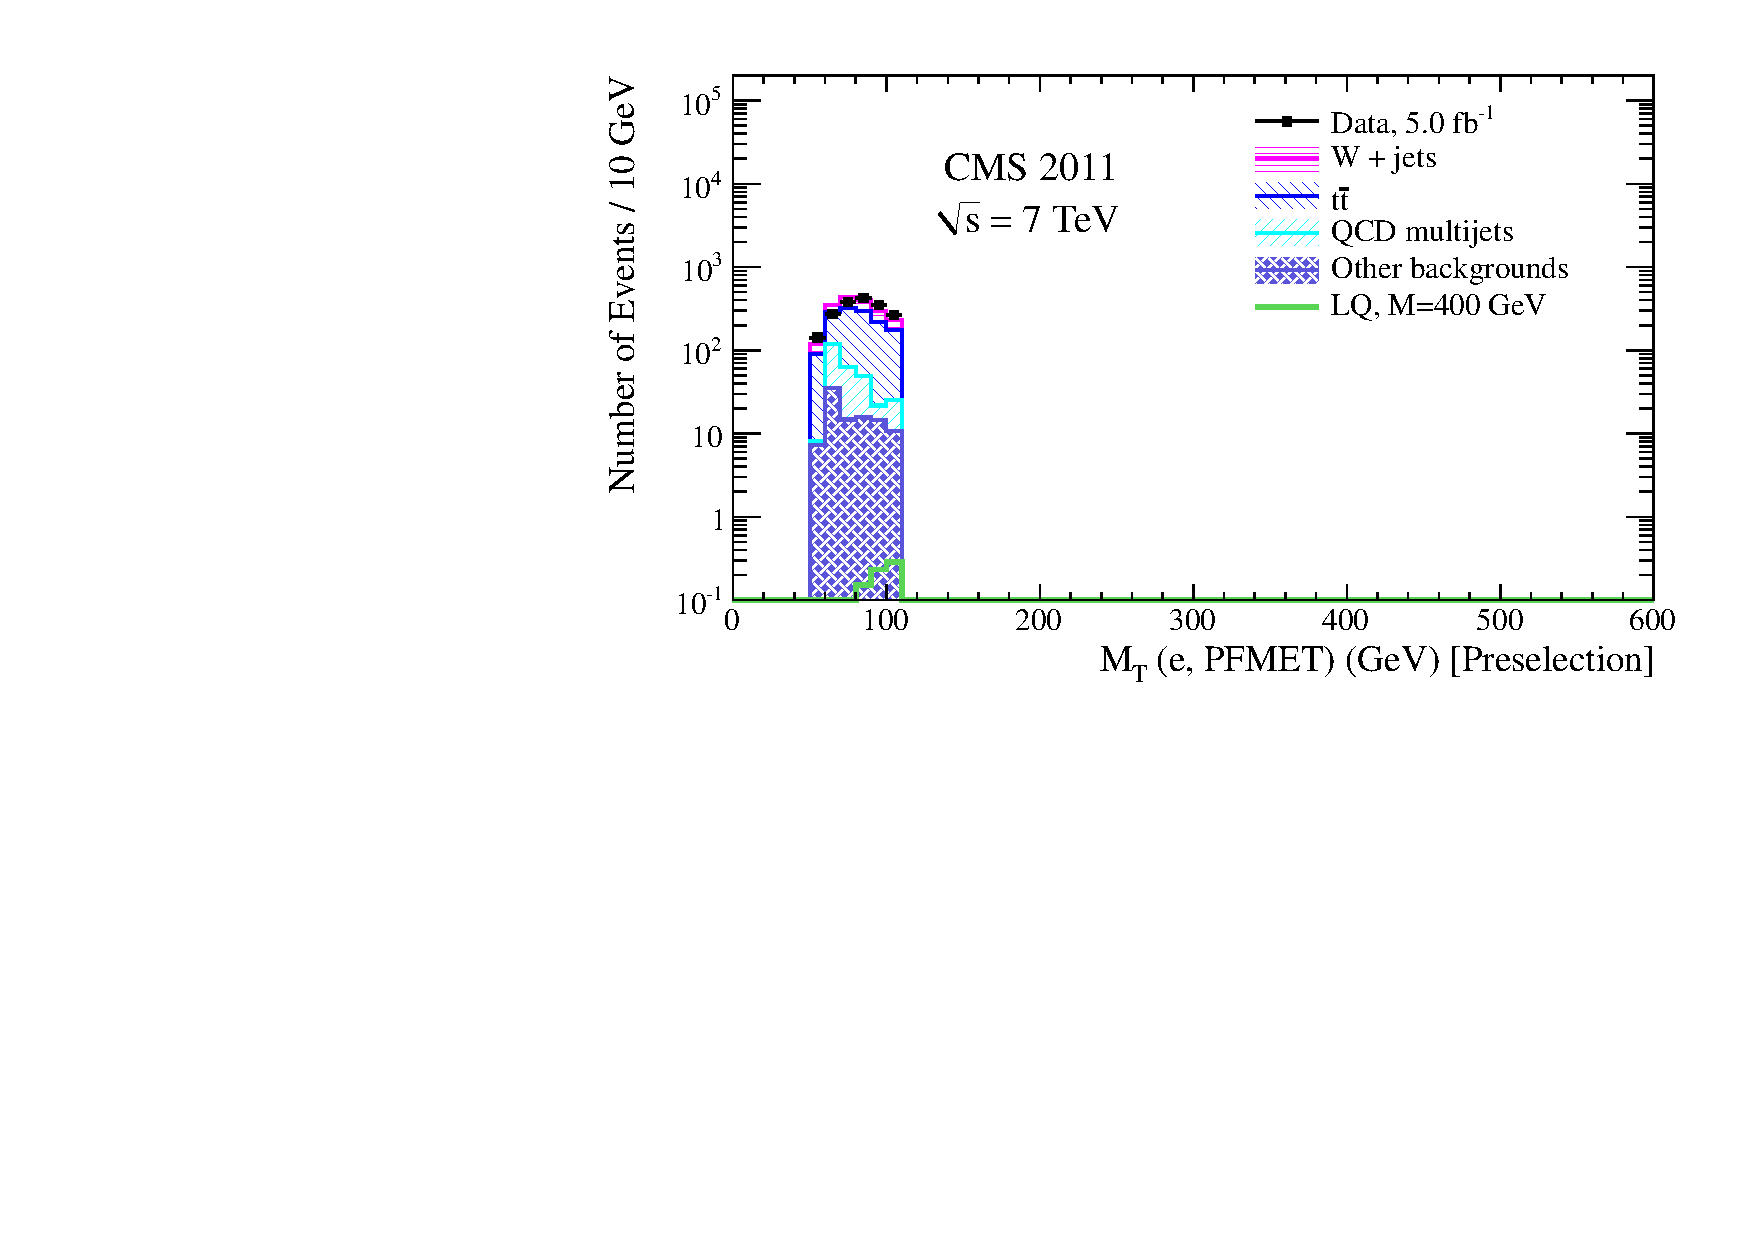
\includegraphics{tex/analysis/backgrounds/fig/MTenu_PAS_enujj_TTBarNorm_5Jets_WZSherpaScaled.pdf}} \\
      \resizebox{7.5cm}{!}{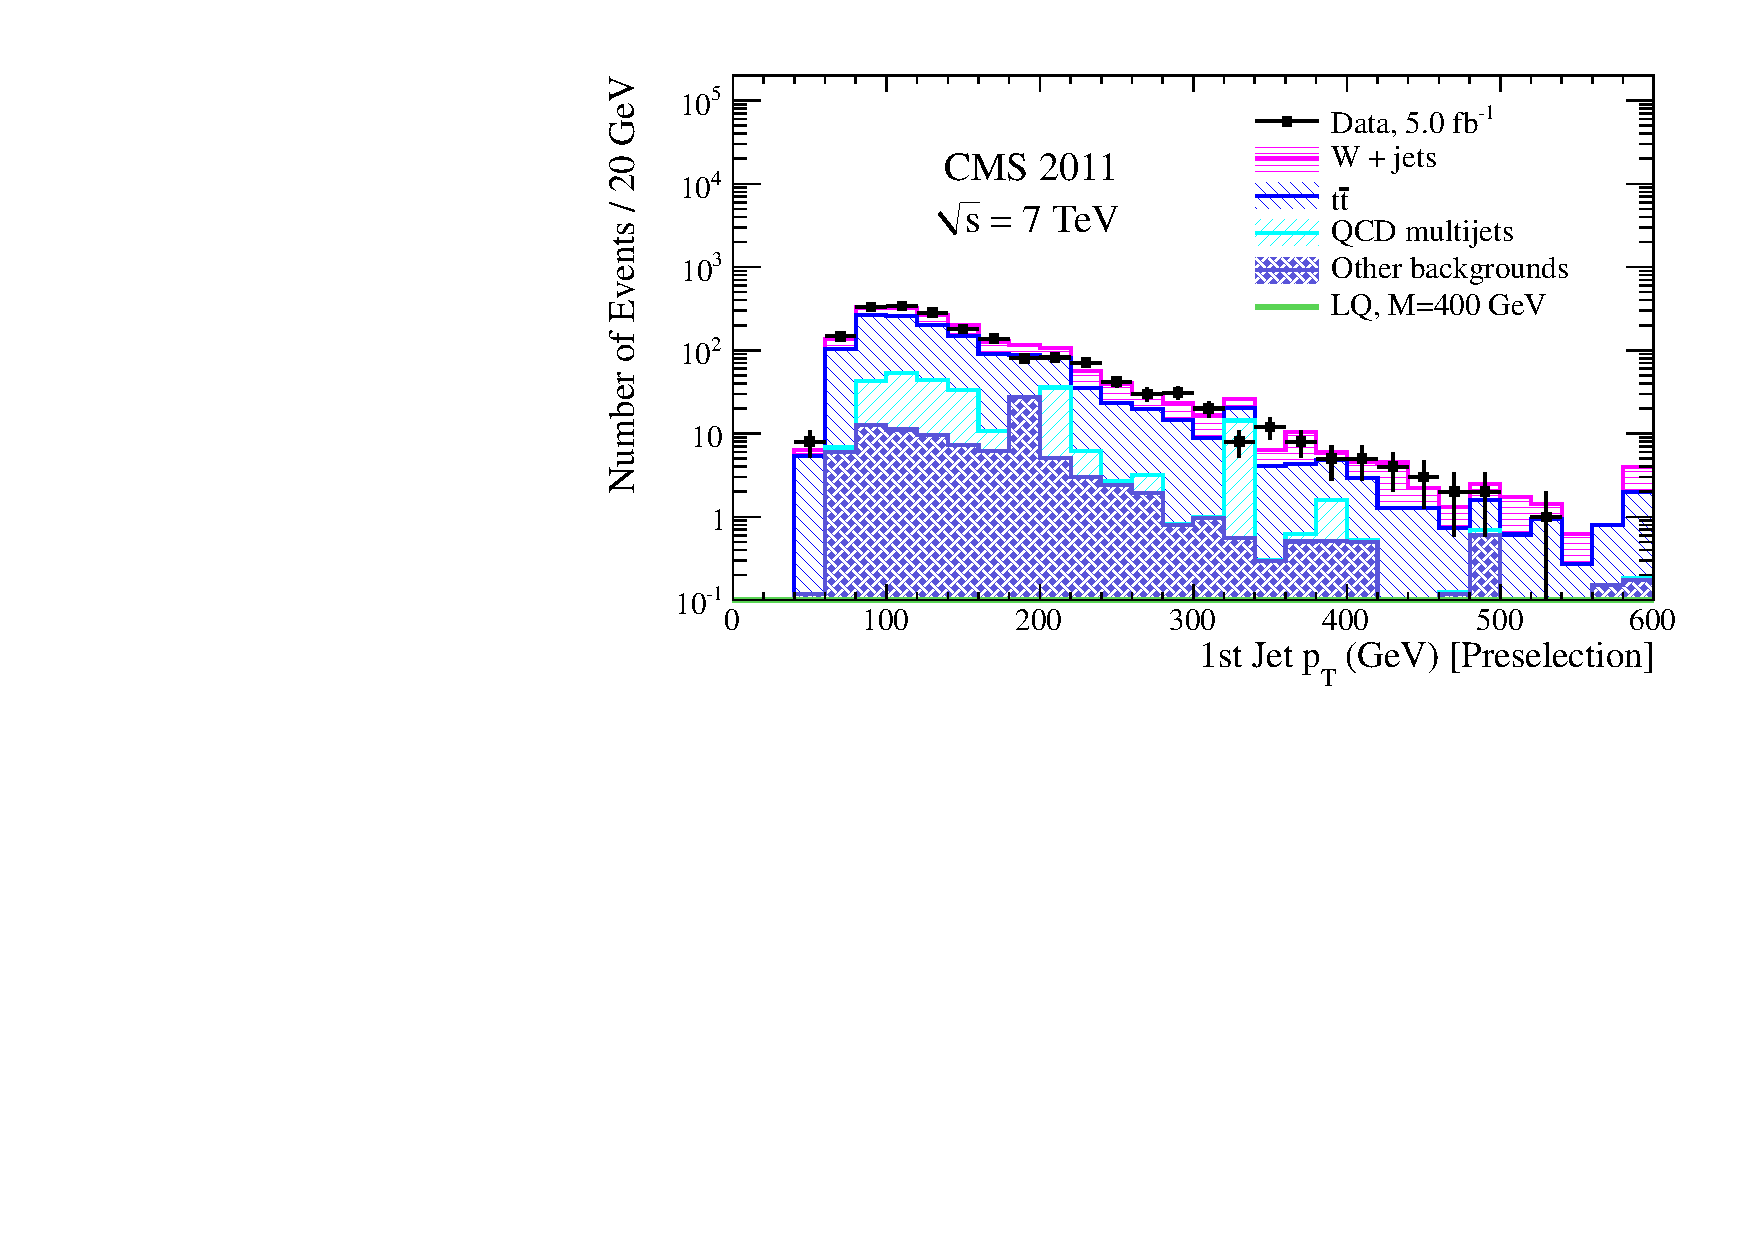
\includegraphics{tex/analysis/backgrounds/fig/Pt1stJet_PAS_enujj_TTBarNorm_5Jets_WZSherpaScaled.pdf}} &
      \resizebox{7.5cm}{!}{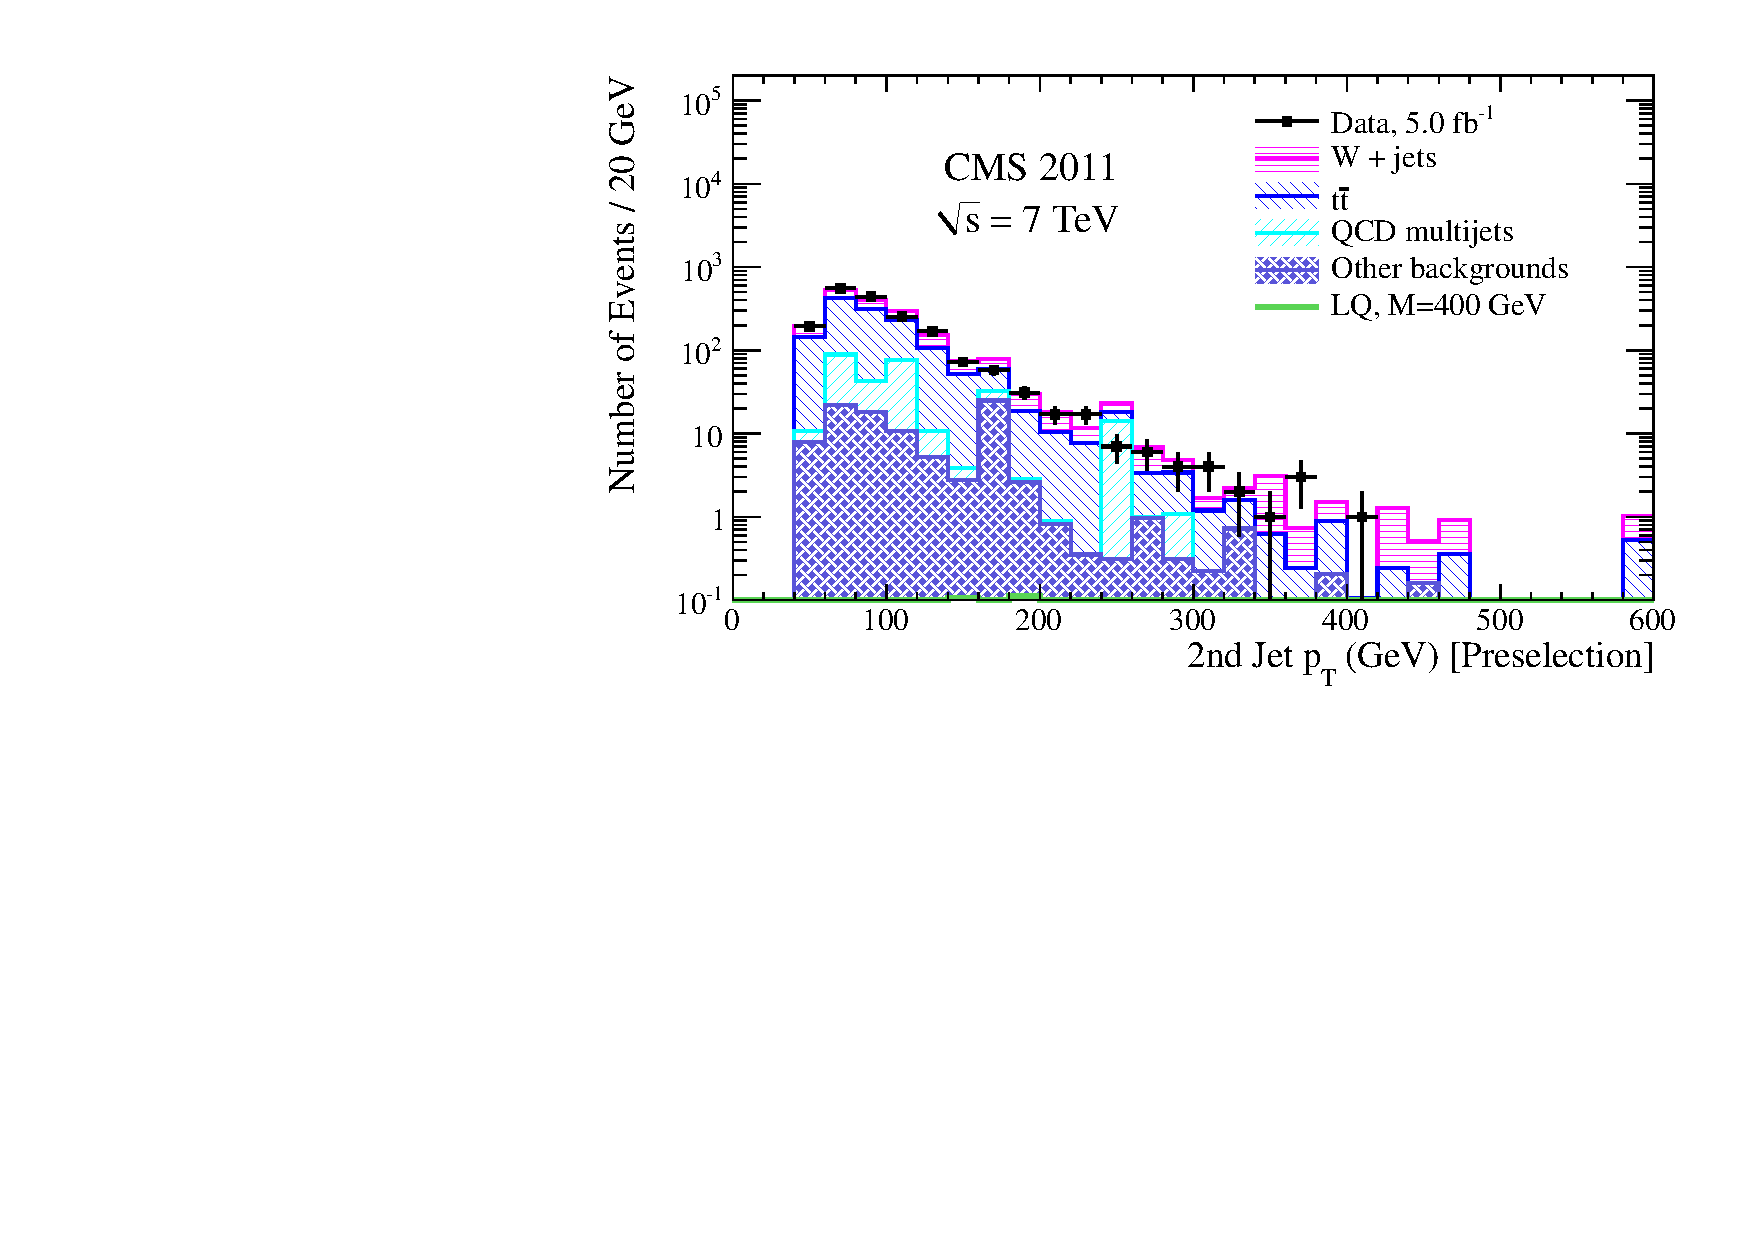
\includegraphics{tex/analysis/backgrounds/fig/Pt2ndJet_PAS_enujj_TTBarNorm_5Jets_WZSherpaScaled.pdf}} \\
      \resizebox{7.5cm}{!}{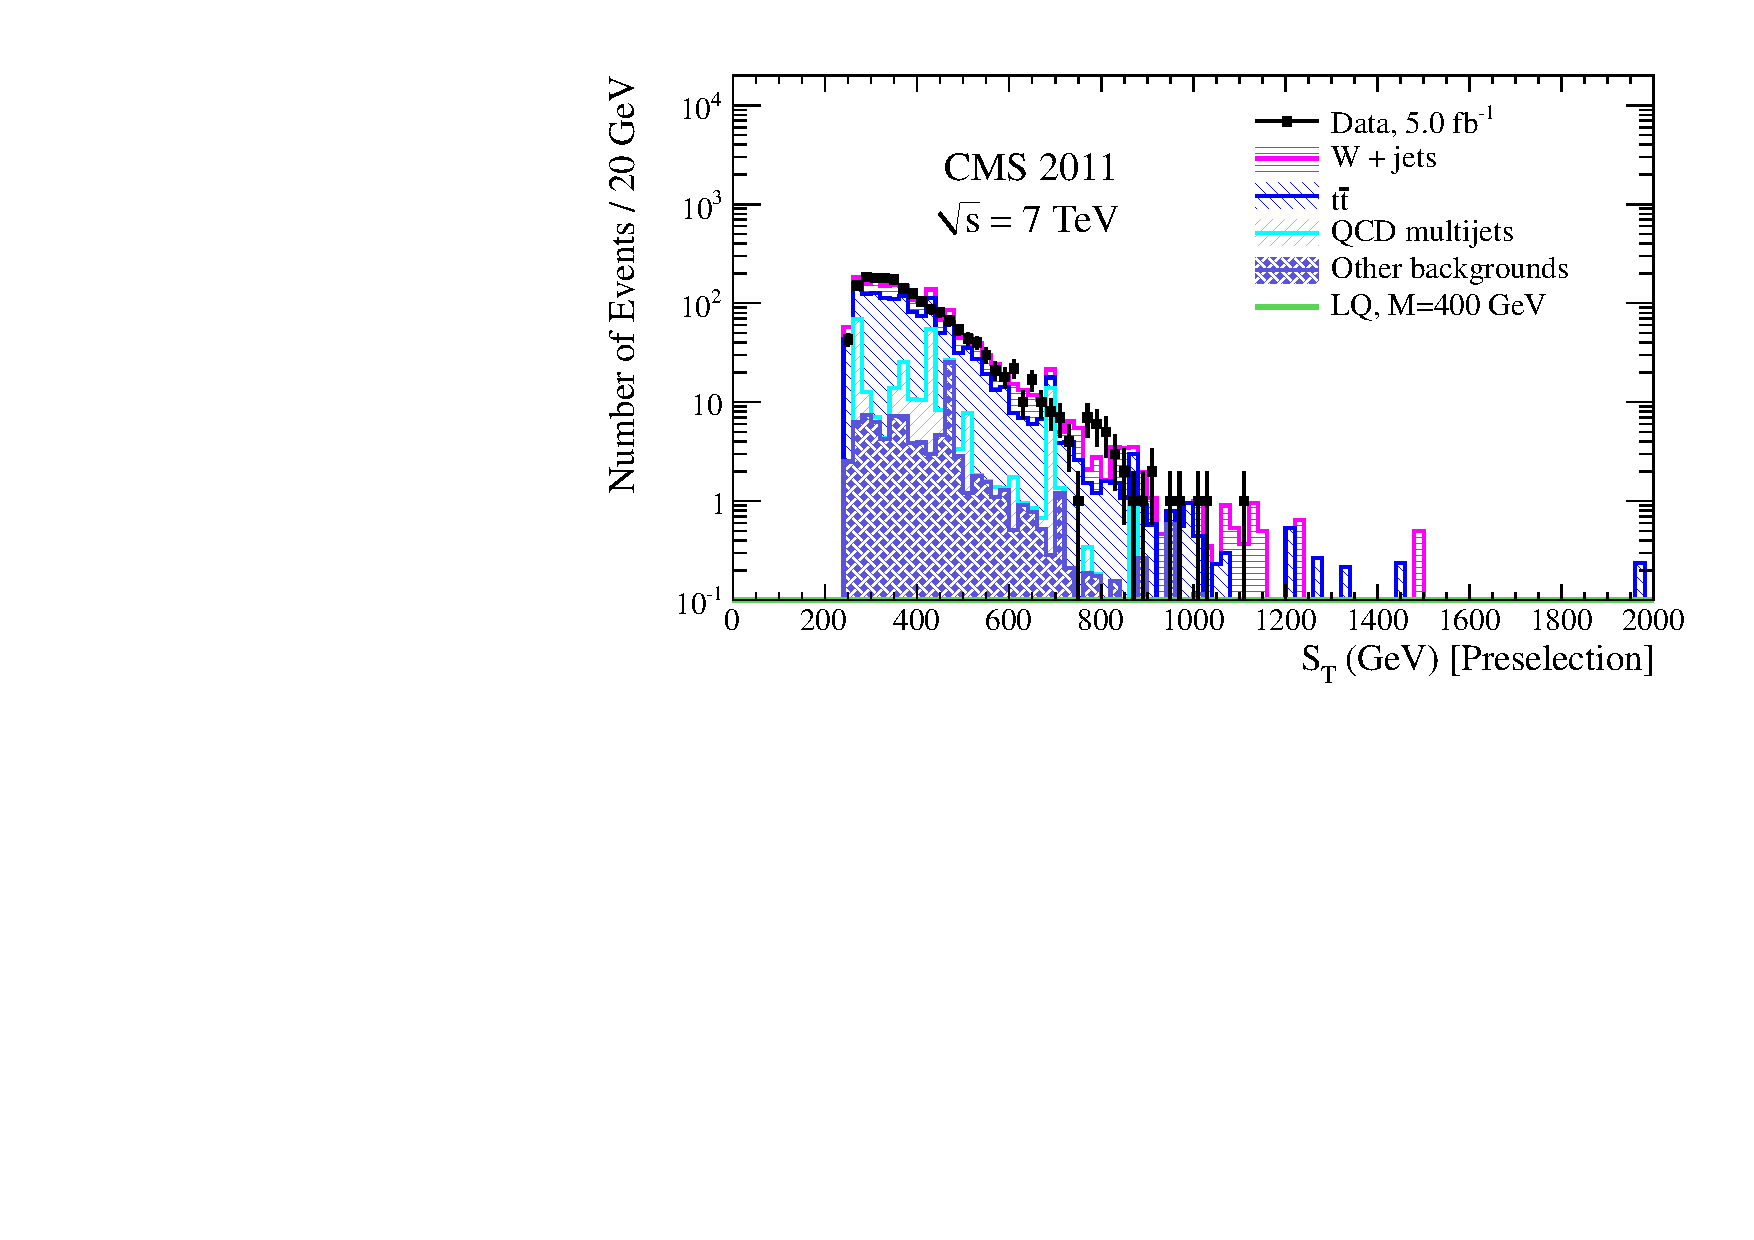
\includegraphics{tex/analysis/backgrounds/fig/sT_PAS_enujj_TTBarNorm_5Jets_WZSherpaScaled.pdf}} &
      \resizebox{7.5cm}{!}{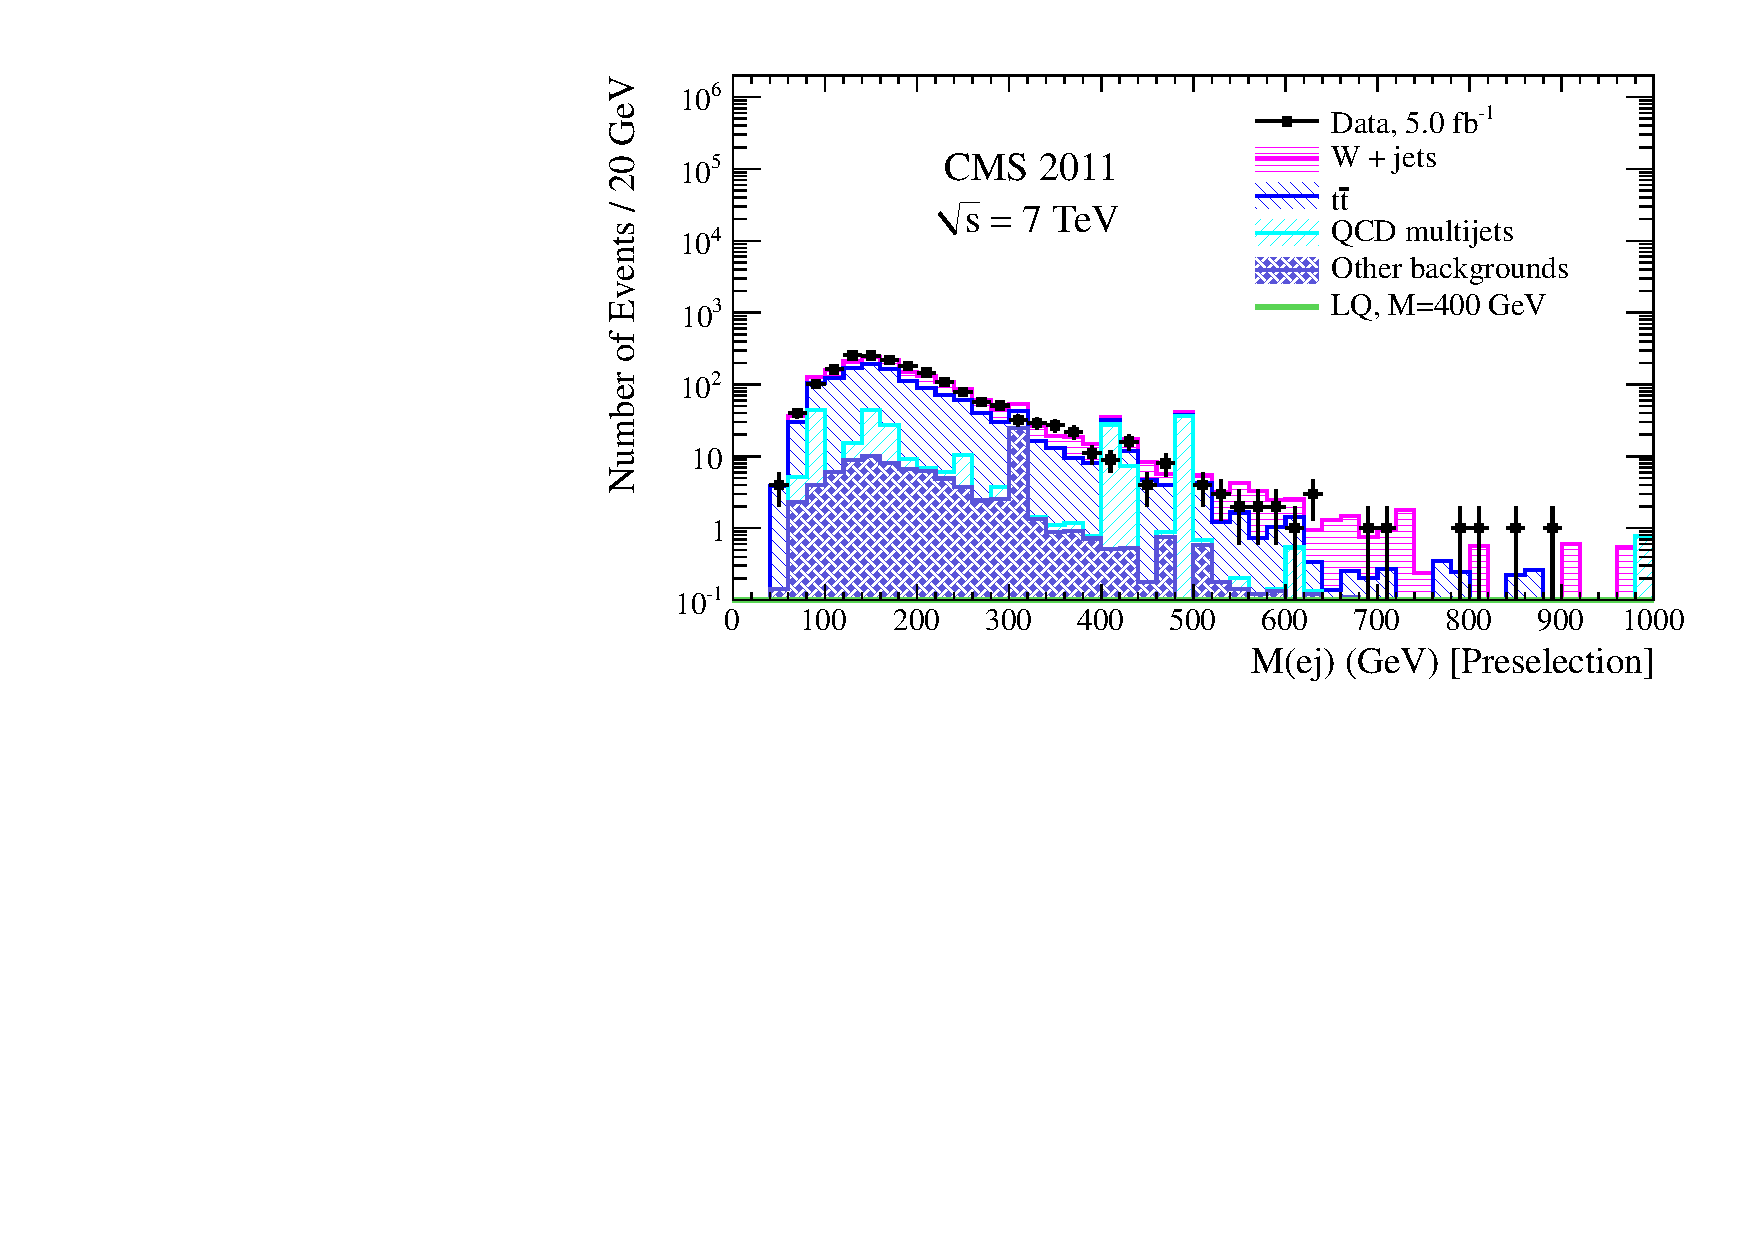
\includegraphics{tex/analysis/backgrounds/fig/Mej_PAS_enujj_TTBarNorm_5Jets_WZSherpaScaled.pdf}} \\
    \end{tabular}
    \caption{The \minptmet~(top left), \mt~(top right), leading jet \pt~(middle left), 
      second leading jet \pt~(middle right), \st~(bottom left), and \mej~(bottom right) 
      distributions for an \enujj~sample enriched in \ttbar~events after the 
      rescaling of this MC background simultaneously with the rescaling of the \wjets~background.}
    \label{fig:manyplots_enujj_ttbarEnriched}
  \end{center}
\end{figure}   
